\documentclass{beamer}

\usetheme{Warsaw}

\usepackage[utf8]{inputenc}
\usepackage[frenchb]{babel}
\usepackage[T1]{fontenc}
\usepackage{amsmath}
\usepackage{hyperref}

\usepackage{graphicx}

\usepackage{tikz}
\usetikzlibrary{arrows}

\pdfcompresslevel0

\usepackage{color}

\addtobeamertemplate{footline}{\hfill\insertframenumber/\inserttotalframenumber
\hspace{10em}\\}

\usepackage{listings}

\title{Interopérabilité entre OCaml et Java }
\author{Béatrice Carré}
\date{\today}

% slides number
\defbeamertemplate*{footline}{shadow theme}
{%
  \leavevmode%
  \hbox{\begin{beamercolorbox}[wd=.5\paperwidth,ht=2.5ex,dp=1.125ex,leftskip=.3cm plus1fil,rightskip=.3cm]{author in head/foot}%
    \usebeamerfont{author in head/foot}\insertframenumber\,/\,\inserttotalframenumber\hfill\insertshortauthor
  \end{beamercolorbox}%
  \begin{beamercolorbox}[wd=.5\paperwidth,ht=2.5ex,dp=1.125ex,leftskip=.3cm,rightskip=.3cm plus1fil]{}%
    \usebeamerfont{title in head/foot}\insertshorttitle%
  \end{beamercolorbox}}%
  \vskip0pt%
}





\begin{document}

\maketitle





\begin{frame}{Comparaison des deux mondes}

intro : interopérabilité : accès Java facile et implicite, gestion
mémoire et exceptions, TODO

\end{frame}



\begin{frame}{Comparaison des deux mondes}
  
L'interopérabilité se fait sur le modèle objet de chacun

\bigskip
\begin{tabular}{|l|c|c|c|c|}
  \hline
  \emph{caractéristiques} & \emph{Java} & \emph{OCaml} \\
  \hline
  accès champs & selon la visibilité & via appels de méthode\\\hline
  var./méth. statiques & \checkmark & fonct./décl. globales\\\hline
  typage dynamique & \checkmark & pas de downcast \\\hline
  héritage$\equiv$sous-typage? &\checkmark  & $\times$ \\\hline
  surcharge & \checkmark & $\times$ \\\hline
  héritage multiple & pour les interfaces & \checkmark\\
  \hline
  packetages/modules & $\emptyset$ mod. paramétrés & \checkmark\\\hline
\end{tabular}

\bigskip

$\Rightarrow$ Il faut réduire les possibilités d'un outil à l'intersection des deux mondes
 
\end{frame}




\begin{frame}{O'Jacaré : schéma global }
Pour un accès à des classes Java :
\medskip
\begin{figure}[h]
  \centering
  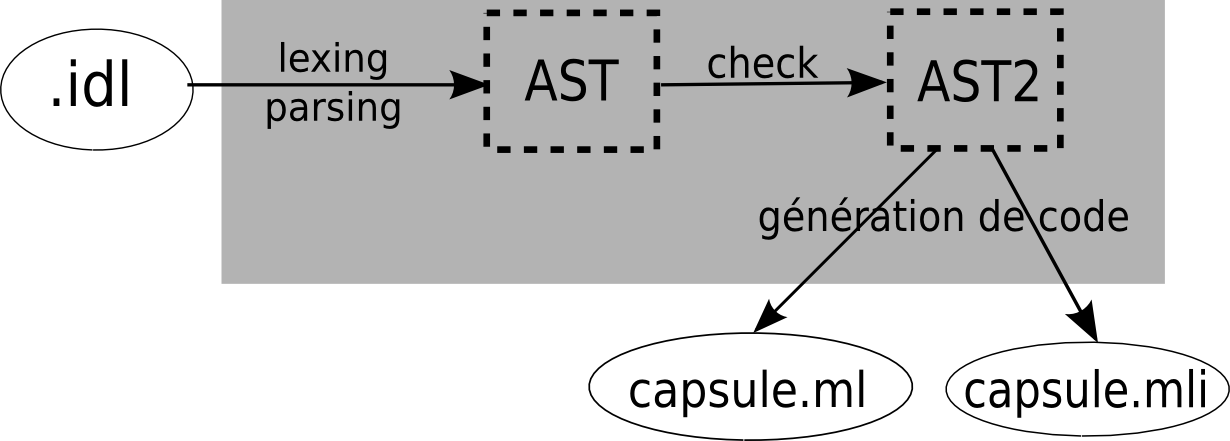
\includegraphics[scale=0.6]{schemaOjacare.png}
  \caption{La génération de code d'O'Jacaré}
\end{figure}
Génération des classes encapsulantes
\end{frame}





\begin{frame}{O'Jacaré : schéma global }
La capsule générée permet à l'utilisateur de faire des appels transparents à des méthodes Java.

Camljava gère la communication entre les deux mondes :
\begin{itemize}
\item Recherche des classes par nom et des méthodes par signature
\item Conversion des types de base est assurée
\end{itemize}
\begin{figure}[h]
  \centering
  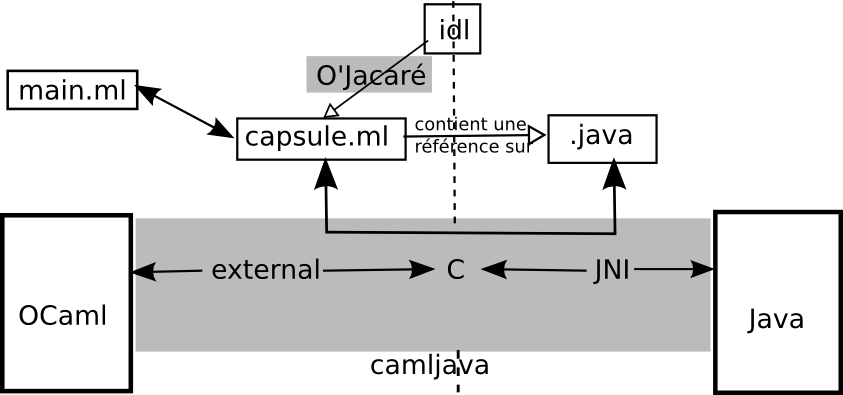
\includegraphics[scale=0.6]{schemaCamljava2.png}
\end{figure}

\end{frame}







\begin{frame}{O'Jacaré : exemple d'idl}
  
\begin{figure}[h]
  \centering
  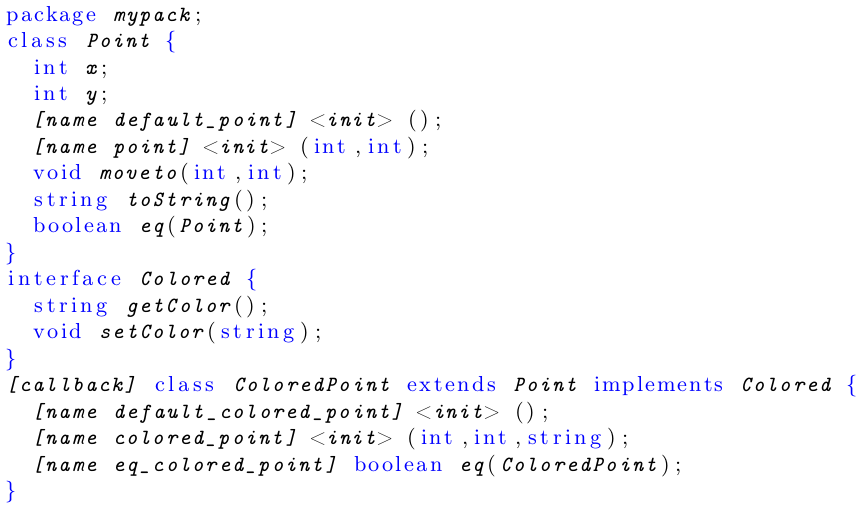
\includegraphics[scale=0.35]{pointIdlEx.png}
\end{figure}
\end{frame}




\begin{frame}{OCaml-Java : schéma global}
\begin{figure}
  \centering
  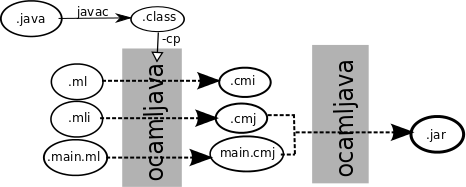
\includegraphics[scale=0.5]{schemaOCamlJava.png}
\end{figure}
Compilation vers du bytecode Java

$\Rightarrow$ un seul runtime
Pas de problème de gestion mémoire, de communications .
\end{frame}

\begin{frame}{OCaml-Java : module OCaml ``Java''}
\begin{tabular}{|l|l|}
  \hline
  type Java & description et exemple \\
  \hline
  java\_constructor & signature d'un constructeur  \\
  &  "java.lang.Object()" \\
  \hline
  java\_method & signature d'une méthode \\
  & "java.lang.String.lastIndexOf(string):int"\\
  \hline
  java\_field\_get & signature d'un attribut\\
  & "mypack.Point.x:int" \\
  \hline
  java\_field\_set & signature d'un attribut\\
  & "mypack.Point.x:int" \\
  \hline
  java\_type & classe, interface ou type Array\\
  & "java.lang.String"\\
  \hline
  java\_proxy & type d'une interface\\
  & "java.lang.Comparable"\\ 
  \hline
\end{tabular}
\end{frame}



\begin{frame}{OCaml-Java : l'accès au monde Java}

\begin{figure}[h]
  \centering
  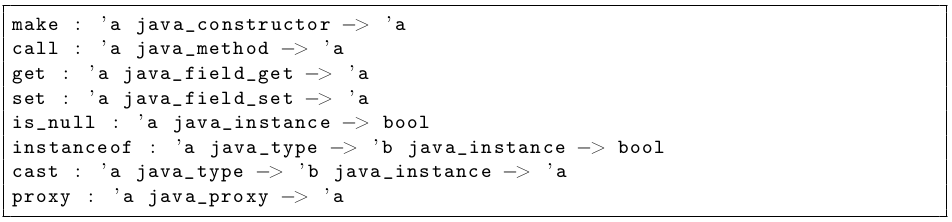
\includegraphics[scale=0.35]{methModuleJava.png}
\end{figure}

Accès à l'API Java et à du code utilisateur grâce à ce module OCaml.




\end{frame}


\begin{frame}{Fusion des deux approches}



\end{frame}




\begin{frame}{Bibliographie}
  
  \begin{thebibliography}{9}
  \bibitem{amato2013localizing}
    Amato, Gianluca and Scozzari, Francesca,
    \emph{Localizing widening and narrowing}.
    Static Analysis, Springer.
    pages 25--42,
    2013.

  \bibitem{halbwachs2012decreasing}
    Halbwachs, Nicolas and Henry, Julien,
    \emph{When the decreasing sequence fails}.
    Static Analysis, Springer.
    pages 198--213,
    2012.
  \end{thebibliography}

\end{frame}

\end{document}

